%%%% INTRODUCTION %%%%
% Motivation for work (from a very general perspective)
\chapter{Introduction}
Virtual navigation of three-dimensional (3D) ambisonics-encoded sound fields (i.e., sound fields that have been decomposed into spherical harmonics) enables a listener to explore an acoustic space (e.g., a concert hall, restaurant, etc.) and, ideally, experience a spatially- and tonally-accurate perception of the sound field.
Applications of this type of virtual sound field navigation (hereafter, just ``virtual navigation'') may be found in virtual-reality (VR) reproductions of real-world spaces.
For example, given an acoustic recording of an orchestral performance, a listener can virtually navigate that recording in order to experience that performance from different vantage points.
Playback of the recording (before of after navigation) may be achieved through a variety of \textit{3D audio} (or, more generally, \textit{spatial audio}) techniques, several of which are described in the following section, which aim to recreate for the listener the spatial characteristics (e.g., placement of sources, reverberation of the space, etc.) of the original sound field.

Another application of virtual navigation can be found in VR games, in which synthetic spatial room impulse responses%
\footnote{A room impulse response (RIR) describes the transmission of sound from a source at a certain position in the room to a receiver at another position in the room and its contents.
Included in the RIR are all reflections, reverberation, and other interactions of the sound with the room.
A \textit{spatial} RIR includes not just the signals that reach the receiver, but also information about the direction of arrival of each signal, thereby preserving the spatial distribution of the incoming sound.}
(RIRs) are used to produce spatial audio.
Since calculating these spatial RIRs often entails computer modeling of complex wave-phenomena and room characteristics, which can be too computationally intensive to perform accurately on-the-fly, it may be preferable to pre-render spatial RIRs on a fixed grid of points and then, in real-time, navigate between them to generate spatial RIRs at intermediate positions.

Virtual navigation may also be ideal for position-constrained, single-listener experiences, such as VR movies.
Unlike large-scale navigable experiences (e.g., in a large room or concert hall), which may require many (e.g., $\sim10+$) microphones to adequately span the space, position-constrained experiences may only require a few (e.g., between 1 and 4) microphones, making this application much more practically feasible.
Additionally, as will be shown in the present thesis, existing navigational methods often perform significantly better when sound sources are far from the microphone(s) compared to the size of the intended navigable region.

%%%% Background and Fundamental Problems %%%%
% Define basic terms in a general sense
% Describe fundamental problems
\section{Background and fundamental problems}\label{sec:01_Introduction:Background}
% define HOA and navigation --> HOA is ideal for navigation
Ambisonics provides a multichannel framework for representing measured 3D sound fields in which each signal (hereafter referred to as an ``ambisonics signal'') represents a different term of that sound field's spherical-harmonic expansion.
Traditionally, a distinction is made between first-order ambisonics (FOA), which uses only the zeroth- and first-order terms of the spherical-harmonic expansion (for a total of four signals), and higher-order ambisonics (HOA), which refers to any expansion beyond first order; the term ``ambisonics'' is used more generally to refer to spherical-harmonic expansions of any order.
The ambisonics signals can be generated synthetically or measured using one or more ambisonics microphones.%
\footnote{Here, we use the term ``ambisonics microphone'' to refer to any array of microphone capsules (typically arranged on the surface of a sphere or tetrahedron) that is used to capture ambisonics signals.
See, for example, \figreftwo{fig:01_Introduction:Eigenmike}{fig:01_Introduction:TetraMic}.}
Generally, virtual navigation aims to generate the appropriate signals for a listener at a point (with any orientation) in a recorded (or synthesized) sound field, such that the resulting perception of the sound field is identical to that which would have occurred in the real sound field.
As will be discussed below, ambisonics representations of sound fields can be manipulated in order to achieve this effect of virtual navigation (i.e., both translation and rotation) of a listener within the captured sound field.

\begin{figure}[t]
\centering
    \begin{subfigure}[b]{0.3\textwidth}
        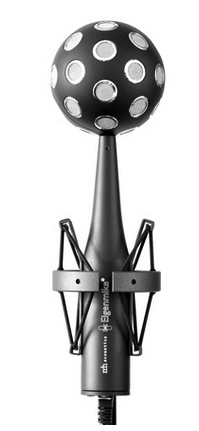
\includegraphics[width=\textwidth]{01_introduction/images/eigenmike_bw.png}
        \caption{Eigenmike}
        \label{fig:01_Introduction:Eigenmike}
    \end{subfigure}
    \hfill
    \begin{subfigure}[b]{0.3\textwidth}
        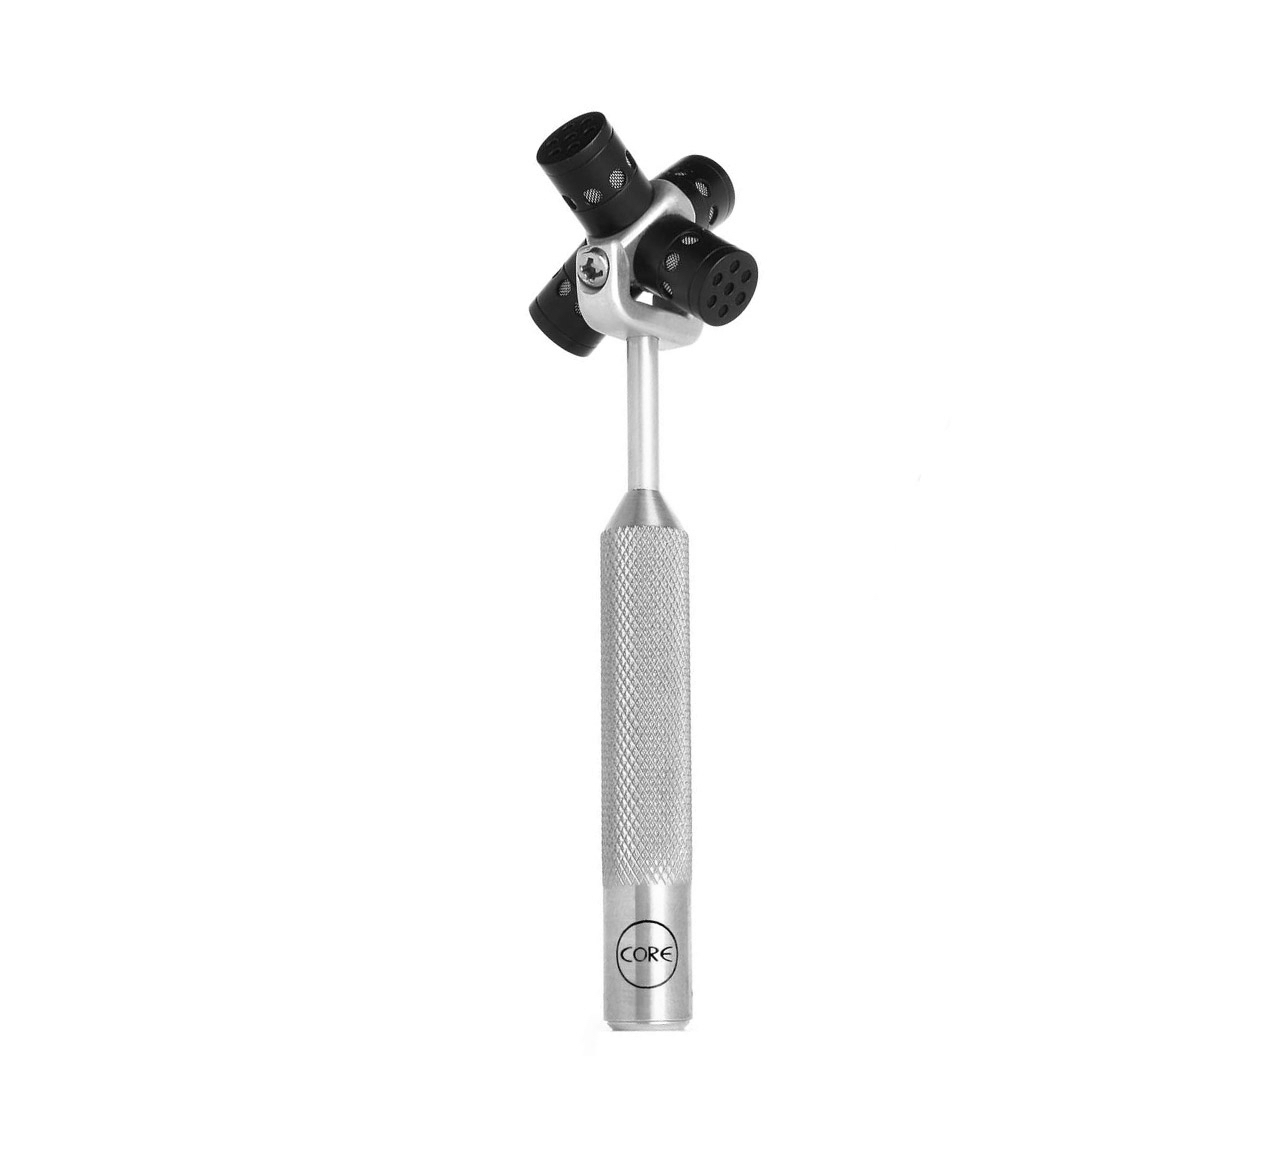
\includegraphics[width=\textwidth,trim={12cm 2cm 12cm 2cm},clip]{01_introduction/images/tetramic_bw.jpg}
        \caption{TetraMic}
        \label{fig:01_Introduction:TetraMic}
    \end{subfigure}
    \hfill
    \begin{subfigure}[b]{0.3\textwidth}
        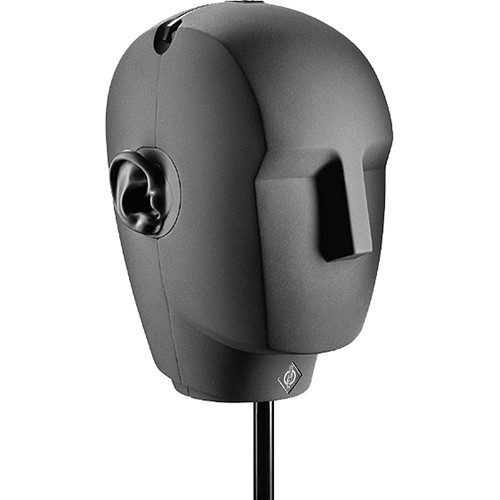
\includegraphics[width=\textwidth,trim={3cm 0 3cm 0},clip]{01_introduction/images/ku100_bw.jpg}
        \caption{KU-100}
        \label{fig:01_Introduction:KU100}
    \end{subfigure}
    \caption[Images of commercially-available spatial audio recording devices.]{
    Images of commercially-available spatial audio recording devices.
    The devices shown are
    the em32 Eigenmike by mh acoustics \citep{EigenmikeURL}, which captures HOA signals;
    the TetraMic by Core Sound \citep{TetraMicURL}, which captures FOA signals; and
    the KU-100 dummy head by Neumann \citep{NeumannKU100URL}, which captures binaural signals.
    }
\end{figure}

% for comparison, binaural has problems
For comparison, traditional binaural recordings (such as those made with a binaural dummy head, an example of which is shown in \figref{fig:01_Introduction:KU100}, or with a pair of small, in-ear microphones placed at the entrances of a human's ear canals) can provide a listener with an accurate spatial perception of a 3D sound field, but are inherently limited in two ways:
\begin{enumerate}
    \item the perspective experienced by the listener during playback is restricted to the vantage point of the recording individual (or device) in the original sound field and
    \item the 3D localization cues (i.e., information used by the human auditory system to determine the origin of a sound) embedded in the recording are only ideally suited for playback to the recording individual, as the recording individual's unique morphology (i.e., that individual's head-related transfer function, or HRTF) has already filtered the incoming sound waves in a highly idiosyncratic and direction-dependent manner.
\end{enumerate}
Examples of such localization cues include the \textit{interaural time difference}, i.e., the signal's time-of-arrival delay between the listener's ears; the \textit{interaural level difference}, i.e., the relative signal amplitudes between the listener's ears; and \textit{spectral cues}, which describe any spectral features added to the incoming sound that originate through interactions with the listener's morphology, e.g., pinnae (outer ears), head, and torso.
For a more thorough review of the fundamentals of sound localization, the interested reader is referred to the works of \citet[chapter 2]{Blauert1997} and \citet[section 1.4]{Xie2013}.

%% multi-binaural solves the rotation problem, but not the individualization problem
A partial solution to the former issue has been developed, known as ``motion-tracked binaural,'' in which multiple binaural signals are recorded (for example, by a roughly head-sized sphere with $\sim8$ microphones spaced around the horizontal-plane circumference) and, during playback, the listener's head rotation is measured and used to select (or compute via interpolation) the appropriate pair of signals \citep{Algazi2004}.
Measuring the listener's head movements is relatively straightforward using commercially-available head-tracking solutions%
\footnote{See, for example, the NaturalPoint TrackIR device (infrared) \citep{TrackIRURL}, the Polhemus Fastrak system (electromagnetic) \citep{PolhemusURL}, and the Visage Face Tracking software (facial recognition) \citep{VisageURL}.} 
and recently, commercial recording devices have been produced which include multiple sets of pinnae in order to produce more realistic binaural signals than those captured by a simple sphere.%
\footnote{See, for example, the 3Dio Omni Binaural Microphone \citep{3DioOmniBinauralURL} and the Hear360 8ball \citep{Hear3608ballURL}.}
This approach, however, can only account for azimuthal (yaw) head rotations; it cannot perform other head rotations (i.e., pitch or roll) or translations of the listener.
Additionally, unless the recording device is physically modified prior to recording to match the listener's particular HRTFs, these solutions fail to address the latter issue of individualization.

%% HOA-to-binaural solves individualization problem; requires HRTFs which are an active area of research
With an ambisonics recording, however, this latter issue can be resolved by post-processing the recorded signals with an individual's particular HRTFs, in a process known as \textit{binaural decoding} (or binaural rendering) of ambisonics.
When played back over headphones,%
\footnote{Alternatively, accurate binaural reproduction can be achieved using appropriately crosstalk-cancelled stereo loudspeaker systems \citep{Choueiri2017a}.}
the listener receives binaural signals that are (ideally) perceptually indistinguishable from those that would have been captured had the listener been physically present in the recorded sound field.
In principle, this approach can accurately produce the necessary 3D localization cues for any listener, although doing so requires accurately measured (or modeled) HRTFs for each listener, which are not trivial to acquire.
Indeed, the acquisition of accurate HRTFs, either through acoustical measurements or computational models, is its own vast and active area of research \citep{Nicol2010,Xie2013}.
Nevertheless, as such HRTF acquisition methods improve, binaural decoding of ambisonics will become ever more practical and accurate.

%% HOA-to-binaural easily performs listener rotation, but translation is more difficult
Existing binaural decoding techniques (several of which are reviewed in \secref{sec:02_Acoustical_Theory:Binaural_Rendering}) have primarily been developed only to place the listener at the position of the recording array \citep{McKeagMcGrath1996,Noisternig2003a,Duraiswami2005a,BergeBarrett2010b,Bernschutz2014} and consequently can only account for listener rotations.
Rotation of the listener (or, equivalently, of the sound field) in ambisonics is straightforward and has been well-established in the literature \citep{GumerovDuraiswami2005,Zotter2009PhD}, so we will not discuss it in detail; briefly, it involves the application of rotation matrices to change coordinates and a frequency-independent mixing of the ambisonics signals (formulae for some such rotation matrices are reproduced here in \secref{sec:A1_Navigation_Filters:Rotation_Matrices}).
In practice, these rotation matrices can be computed and applied in real-time based on the measured orientation of the listener's head.
Translations of the listener can also be performed in real-time based on either the measured position of the listener (e.g., from a head-tracking device) or some other user input, such as from a video game controller.
Methods to translate the listener, however, entail more complex processing and are not as well-established, nor have the penalties incurred by such processing been fully characterized.

%% translation is limited by theory and results in coloration & localization errors, but higher orders are better
Translation of the listener is made difficult by a well-known limitation of the ambisonics framework: that a finite-order expansion of a sound field yields only an approximation to that sound field, the accuracy of which decreases with increasing frequency and distance from the expansion center \citep{Poletti2005,WardAbhayapala2001}.
In particular, a well-established rule of thumb states that a sound field is accurately represented%
\footnote{Specifically, \citet{WardAbhayapala2001} show that obeying the inequality given in \eqnref{eq:01_Introduction:kr_Inequality} yields a \textit{reconstruction error} (i.e., the discrepancy between the exact pressure field and its order-limited approximation) of at most 4\%, which the authors claim ``should be sufficient for most practical applications.''}
by an $L^\textrm{th}$-order expansion up to a distance $r$ provided that
\begin{equation}\label{eq:01_Introduction:kr_Inequality}
kr \leq L,
\end{equation}
where $k$ is the angular wavenumber \citep[Eq.~(17)]{WardAbhayapala2001}
(cf.~\citet[Eq.~(28)]{Poletti2005} and \citet[p.~289]{Nicol2017}).
As a consequence, existing extrapolation-based navigational methods (hereafter referred to as \textit{extrapolation} methods,%
\footnote{In this thesis, we distinguish between two categories of navigational methods: \textit{extrapolation} methods, which employ only a single ambisonics microphone, and \textit{interpolation} methods, which employ an array of ambisonics microphones distributed throughout the sound field (or, equivalently, take samples at multiple discrete positions throughout a synthetic sound field).}
several of which are reviewed in \secref{sec:03_Navigation_Techniques:Extrapolation_Methods}) have been shown to introduce spectral coloration (i.e., audible changes in the spectral content of a signal) \citep{KuntzRabenstein2007,HahnSpors2015b} and localization errors (i.e., errors in the perceived direction of a sound relative to the listener) \citep{Winter2014,TylkaChoueiri2015} as the listener navigates farther away from the expansion center.%
\footnote{Similar results were found by \citet{WaltherFaller2010}, although their aim was not to navigate the sound field, but instead to simulate a spaced-microphone recording using a single first-order ambisonics microphone.}
However, previous studies have also shown (and we will also show here in \chapref{chap:07_Characterization_Extrapolation}) that these penalties decrease as the expansion order of the recording increases \citep{Winter2014,TylkaChoueiri2015}.
Thus, since synthetic sound fields can be generated to arbitrarily high orders, and since microphone array technology is rapidly advancing, it may soon be practical to capture very high-order expansions of real sound fields, thereby increasing the viability of extrapolation methods.

%% near-field sources, however, require additional steps
Another more fundamental limitation of the ambisonics description of sound fields is that the region over which the spherical-harmonic expansion is \textit{valid} is restricted by the nearest sound source or scattering body to the expansion center, so near-field sources and obstacles pose a particularly limiting problem to virtual navigation (see \secref{sec:02_Acoustical_Theory:Helmholtz_Equation} for a review of the relevant acoustical theory).
Although many sound fields are free of extremely near-field sources and obstacles, many of interest are not, so additional steps must be taken to overcome this limitation.
For example, if the near-field sources in a sound field can be identified, localized, and isolated from the rest of the recording, then they can be processed and rendered separately, thereby enlarging the effective region of validity for navigation.

%% broadly discuss recent developments (and introduce categorizations)
In recent work, \textit{parametric} navigational methods%
\footnote{So-called \textit{parametric} navigational methods are those that depend on additional information (e.g., source positions) beyond the ambisonics input signals in order to perform the navigation.
That is, the particular processing carried out by these methods directly depends on some such parameter of the sound field.
For \textit{linear} methods, on the other hand, all relevant parameters (e.g., virtual loudspeaker positions) may be specified offline, so the processing carried out during playback is independent of any changes to the sound field.}
have been developed to overcome this restriction by leveraging additional information about the positions of sources \citep{TylkaChoueiri2016,Wakayama2017}.
Additionally, navigational methods that employ multiple ambisonics microphones (hereafter referred to as \textit{interpolation} methods, several of which are reviewed in \secref{sec:03_Navigation_Techniques:Interpolation_Methods}) enable navigation near to and around such near-field sources \citep{TylkaChoueiri2016,Thiergart2013,Zheng2013PhD} (as will be shown in \chapreftwo{chap:08_Proposed_Method}{chap:09_Thiergart_Comparison}), although published findings on this subject are limited.
Existing navigational methods are summarized in \tabref{tab:01_Introduction:Methods}.

\begin{sidewaystable}
\centering
\begin{tabular}{l|c|c|c|l}
\textbf{Method} & \textbf{Processing} & $P$ & $L_\textrm{in}$ & \textbf{Additional Inputs} \\\hline\hline
Virtual ambisonics \citep[section 3.1]{TylkaChoueiri2015} & Linear & 1 & $1+$ & \\\hline
Plane-wave translation \citep{SchultzSpors2013} & Linear & 1 & $1+$ & \\\hline
Ambisonics translation \citep{GumerovDuraiswami2005,MenziesAlAkaidi2007a,Zotter2009PhD} & Linear & 1 & $1+$ & \\\hline
Singular ambisonics translation \citep{Wakayama2017} & Parametric & 1 & $1+$ & Source position \\\hline
Distance-mapped sound field modeling \citep{Plinge2018} & Parametric & 1 & 1 & Distance map of environment \\\hline
Spherical equivalent source method \citep{FernandezGrande2016} & Linear & $1+$ & $1+$ &  \\\hline
Inverse ambisonics translation via plane-waves \citep{WangChen2018} & Linear & $1+$ & $1+$ &  \\\hline
Sparse plane-wave estimation and translation \citep{Emura2017} & Nonlinear & 2 & $1+$ &  \\\hline
Weighted-average interpolation \citep{Southern2009,MarietteKatz2009} & Linear & $2+$ & $1+$ &  \\\hline
Regularized inverse ambisonics interpolation \citep{Samarasinghe2014a,TylkaChoueiri2016,Ueno2018} & Linear & $2+$ & $1+$ &  \\\hline
Distance-biased linear interpolation \citep{Patricio2019} & Linear & $2+$ & $1+$ &  \\\hline
Dynamic time warping RIR interpolation \citep{Masterson2009,Kearney2009} & Nonlinear & $2+$ & $1+$ & Source positions \\\hline
Valid-only interpolation \citep{TylkaChoueiri2016} & Parametric & $2+$ & $1+$ & Source positions \\\hline
Time-frequency analysis and modeling \citep{Thiergart2013} & Parametric & $2+$ & 1 &  \\\hline
Collaborative blind-source separation \citep{Zheng2013PhD} & Parametric & $2+$ & 1 &  \\\hline
Perspective control ambisonics microphone array \citep{Bates2018} & Parametric & 4 & $1+$ & 
\end{tabular}
\caption[Summary of published navigational methods.]{
Summary of published navigational methods.
Here, $P$ denotes the number of ambisonics microphones used in the method and $L_\text{in}$ denotes the required ambisonics order of the microphone(s).}
\label{tab:01_Introduction:Methods}
\end{sidewaystable}

% Review previous work focusing on the remaining problems (questions or deficiencies) the present paper claims to contribute to solving
\section{Previous work and remaining problems}
% metrics problem - POMA paper, Ch. 5
As mentioned above, numerous methods for virtual navigation have been developed, many of which have been shown to introduce localization errors \citep{Winter2014,TylkaChoueiri2015,TylkaChoueiri2016} and/or spectral coloration \citep{HahnSpors2015b,TylkaChoueiri2016}.
Although subjective testing is the most direct means of evaluating and comparing navigational methods in terms of these perceptual attributes, such tests are often lengthy and costly, which motivates the use of objective metrics that enable quick assessments of navigational methods.
Existing perceptually-motivated objective metrics often rely on computational models of the human auditory system (so-called ``binaural models'') in order to predict some aspect of the perception of a sound (e.g., perceived source position or spectral content) by a ``typical'' human listener.
Such metrics necessarily conflate the effects of the navigational method with those of the adopted ambisonics-to-binaural rendering approach.
On the other hand, purely signal- or physics-based metrics may circumvent this issue by evaluating the signals prior to rendering to binaural, but they are not necessarily perceptually relevant, in that their predictions may not correspond with subjective listening test responses.
Consequently, suitable (i.e., perceptually relevant and non-binaural) objective metrics for at least coloration and localization are needed in order to both compare existing navigational methods and develop future ones.

% simulation framework - Ch. 6 --> 10
Additionally, each study that has previously attempted to quantify the incurred perceptual penalties often only examined a single navigational method, considered a limited range of conditions (e.g., sound field geometry, input ambisonics order, etc.), and employed a unique set of objective metrics, thus making comparisons across studies essentially impossible.
In order to draw meaningful comparisons between competing navigational methods, a consistent and comprehensive set of tests should be designed and conducted for all existing and future methods.

% comparison of extrapolation methods and quantification of validity penalties - Ch. 7
With the exception of the plane-wave translation method of \citet{SchultzSpors2013} (which we review in \secref{sec:03_Navigation_Techniques:PW_Technique}), most existing extrapolation methods have not been evaluated in terms of perceptual attributes (i.e., coloration and localization).
In particular, any errors related to the region of validity restriction (which all linear extrapolation methods are prone to violate if the listener navigates beyond a near-field source) have not been well-established in the literature.
Additionally, the penalties incurred by different methods have only been directly compared over a limited range of conditions \citep{TylkaChoueiri2015}, making it difficult to choose the appropriate method for a particular application.
Consequently, the performance of existing extrapolation methods should be characterized and compared, and the errors incurred by violating the region of validity restriction should be quantified.

% quantification of validity penalties for interpolation methods - AES 2016 AVAR Paper, Ch. 8
Parametric and interpolation methods may provide adequate solutions to the region of validity restriction, but this issue has not been explored much in the literature.
The simplest existing interpolation method entails a weighted average of the ambisonics signals from different microphones \citep{Southern2009} and (as we will show in \secref{sec:08_Proposed_Method:Fundamental_Problems}) is consequently prone to comb-filtering-like effects and skewed localization due to the precedence effect.
An alternative, least-squares interpolation method may mitigate these issues \citep{Samarasinghe2014a}, but remains prone to violating the region of validity restriction if the sound field contains any near-field sources.
Consequently, in a recent publication, we proposed a parametric interpolation method which ensures that this restriction is not violated \citep{TylkaChoueiri2016}.
Additionally, a recently-proposed parametric extrapolation method circumvents this restriction using \textit{a priori} information of the source positions \citep{Wakayama2017}, and other parametric methods have been developed that construct a navigable model of the incident sound field via a time-frequency analysis \citep{Thiergart2013,Zheng2013PhD,Plinge2018}, and should consequently be immune to this restriction.
However, the performance of these methods has not been fully characterized in terms of perceptual criteria and, in particular, the penalties incurred by violations of the region of validity restriction have not been established.

% comparison of parametric methods - Ch. 9
Finally, the suitability of such methods for different applications has not been established.
For example, while recently-developed parametric methods may yield more accurate localization than linear methods, even in the presence of near-field sources, they have been shown to introduce minor degradations of sound quality \citep[section 5.3]{Zheng2013PhD} and they may not be suitable for dense or highly-reverberant environments \citep[section II]{Thiergart2013}.
Consequently, based on a broad performance characterization of existing parametric interpolation methods, recommendations should be made regarding the suitability of each method to various applications.

%%%% Objectives and Approach %%%%
% A statement of the paper's main question(s) and goal(s), followed by a succinct description of the general method and approach to be described in the paper
\section{Objectives and approach}
It is the overall objective of this thesis to investigate the limitations of, and penalties incurred by, various methods for virtual sound field navigation.
Of particular interest are those penalties relating to a violation of the region of validity restriction.
To these ends, we first develop, and subsequently validate through subjective listening experiments, perceptually-relevant objective metrics for perceived spectral coloration and source localization errors introduced by navigational methods. % Ch. 5
We then design, and later experimentally validate, a numerical simulation framework based on simple incident sound fields, which enables a consistent and comprehensive performance characterization (in terms of a suite of perceptually-relevant objective metrics) across navigational methods. % Ch. 6
To validate these simulations, we perform a set of acoustical measurements taken over a subset of the simulated conditions and determine the magnitudes of any discrepancies in the resulting values of each objective metric. % Ch. 10

Next, we characterize the performance of existing extrapolation methods in order to identify regimes in which each method performs well and to provide insight into the types and severities of incurred penalties under a range of conditions. % Ch. 7
We then revise our previously-proposed parametric interpolation method \citep{TylkaChoueiri2016} in order to mitigate its induced spectral coloration and to characterize and compare the performance of this method and that of a benchmark linear method. % Ch. 8
Similarly, we characterize and compare the performance of an existing parametric time-frequency interpolation method and our revised method. % Ch. 9
From each of these characterizations, we seek broader insights into the nature of the penalties incurred by violating the region of validity restriction and identify considerations regarding the suitability of each method to various applications. % Ch. 11

% A brief section by section description of the structure of the paper
\section{Thesis overview}
The remainder of the present thesis is organized as follows.
The next three chapters consist largely of review material:
\begin{itemize}
\item in \chapref{chap:02_Acoustical_Theory}, we review relevant concepts from acoustics and ambisonics theory;
\item in \chapref{chap:03_Navigation_Techniques}, we review several existing navigational methods; and
\item in \chapref{chap:04_Auditory_Models}, we review existing objective metrics and auditory models.
\end{itemize}
Then, in \chapref{chap:05_Proposed_Models}, we propose auditory models for spectral coloration and localization, describe experiments for their subjective validation, and present corresponding results.
Next, in \chapref{chap:06_Simulation_Framework}, we present the numerical simulation framework employed in subsequent chapters to characterize and compare navigational methods.
The following three chapters consist largely of performance characterizations:
\begin{itemize}
\item in \chapref{chap:07_Characterization_Extrapolation}, we characterize and compare the performance of two existing linear extrapolation methods, and identify penalties incurred by violating the region of validity restriction;
\item in \chapref{chap:08_Proposed_Method}, we revise our previously-proposed parametric interpolation method, and characterize and compare its performance and that of a benchmark linear method; and
\item in \chapref{chap:09_Thiergart_Comparison}, we characterize and compare the performance of an existing parametric interpolation method and our proposed method, and identify suitable domains for the practical application of each method.
\end{itemize}
We then present, in \chapref{chap:10_Experimental_Validation}, an experimental validation of the numerical simulation framework described in \chapref{chap:06_Simulation_Framework}.
Finally, in \chapref{chap:11_Conclusions}, we summarize the major findings from this work; synthesize these findings into a) broader insights regarding the penalties incurred by violating the region of validity restriction and b) guidelines regarding the practical application of each method; and propose avenues for future research.

\section{Relevant prior publications}
Many of the chapters and appendices in this thesis are largely based on the following prior publications by the present author:
\begin{itemize}
\item \chapref{chap:05_Proposed_Models} -- \citet{TylkaChoueiri2017a}
\item \chapref{chap:07_Characterization_Extrapolation} -- \citet{TylkaChoueiri2015} and \citet{TylkaChoueiri2019c} (submitted)
\item \chapref{chap:08_Proposed_Method} -- \citet{TylkaChoueiri2016} and \citet{TylkaChoueiri2019b} (submitted)
\item \chapref{chap:09_Thiergart_Comparison} -- \citet{TylkaChoueiri2019d} (submitted)
\item \chapref{chap:10_Experimental_Validation} -- \citet[section 6]{TylkaChoueiri2019b} (submitted)
\item \apxref{chap:A1_Navigation_Filters} -- \citet{TylkaChoueiri2019a}
\item \apxref{chap:A2_SABRE_Toolkit} -- \citet{TylkaChoueiri2017b}
\item \apxref{chap:A3_Smoothing_Weights} -- \citet*{Tylka2017}
	\begin{itemize}
	\item I performed all of the analysis presented in this publication, although Prof.~Boren conducted some of the initial investigations into the issue, and together we had several fruitful discussions to better identify the problem and which led to the development of the presented smoothing method.
	\end{itemize}
\item \apxref{chap:A4_HRTF_Measurements} -- \citet*{Sridhar2017}
	\begin{itemize}
	\item Mr.~Sridhar was responsible for all of the work on morphological scans described in this publication, but this work is omitted in this appendix.
	Mr.~Sridhar and I contributed equally to the construction of the experimental hardware used to measured the HRTFs, and to the development of the data acquisition and analysis software.
	\end{itemize}
\item \apxref{chap:A5_Impulse_Response} -- \citet*{Tylka2014}
	\begin{itemize}
	\item Mr.~Sridhar and I contributed equally to the development of the presented iterative method and to the experiments and analyses presented in this publication, although only the introductory and background sections, which I have significantly revised, are reproduced in this appendix.
	Prof.~Boren conducted some of the initial investigations into the issue and provided guidance towards the overall direction of the research.
	\end{itemize}
\end{itemize}
Except where noted otherwise, all of the work presented in the papers listed above is my own, with Prof.~Choueiri serving in an advisory capacity and lending guidance towards the overall direction of the research.